\documentclass[letterpaper]{article} % DO NOT CHANGE THIS
\usepackage[submission]{aaai2027}  % DO NOT CHANGE THIS
\usepackage[hyphens]{url}  % DO NOT CHANGE THIS
\usepackage{graphicx} % DO NOT CHANGE THIS
\urlstyle{rm} % DO NOT CHANGE THIS
\def\UrlFont{\rm}  % DO NOT CHANGE THIS
\usepackage{natbib}  % DO NOT CHANGE THIS AND DO NOT ADD ANY OPTIONS TO IT
\usepackage{caption} % DO NOT CHANGE THIS AND DO NOT ADD ANY OPTIONS TO IT
\frenchspacing  % DO NOT CHANGE THIS

\usepackage{amsmath}
\usepackage{amssymb}
\usepackage{booktabs}

\pdfinfo{
/TemplateVersion (2027.1)
}

\setcounter{secnumdepth}{0}

\newcommand{\base}{HARP-GNN}
\newcommand{\esep}{HARP-ESep}
\newcommand{\method}{HARP-Select}
\newcommand{\papertablesize}{\footnotesize}

\title{\method: Confidence-Calibrated Residual Polynomial Experts for Heterophilous Graphs}
\author{
    Anonymous Authors
}
\affiliations{
    Anonymous Affiliation
}

\begin{document}
\maketitle

\begin{abstract}
Graph neural networks for node classification must often operate on graphs whose neighborhoods mix homophilous smoothing evidence with heterophilous contrastive evidence.
This paper studies a simple residual polynomial design for that setting.
We first construct \base, which combines low-pass propagated features with high-pass residual differences through a node-wise gate.
Systematic diagnostics reveal a specialization boundary: self-loop residual filtering is strong on WebKB-style graphs, while an ego-separated no-self variant, \esep, is much stronger on several larger heterophily benchmarks.
We therefore introduce \method, a validation-calibrated expert selector that trains both residual polynomial experts and selects \esep{} only when its validation advantage exceeds a fixed normal-approximation uncertainty threshold.
The rule uses validation labels only, is frozen across datasets, and exposes every per-split decision.
Across six fixed-split heterophily benchmarks, \method{} removes the significant Chameleon and Squirrel deficits of \base{} while preserving its Texas and Wisconsin behavior; robust paired checks indicate branch specialization rather than unbounded leaderboard dominance.
On external critical-heterophily graphs, \esep{} improves Roman-Empire by 2.75 percentage points under paired tests and the frozen selector routes all splits to it, while conservatively retaining \base{} on Amazon-Ratings.
The resulting contribution is an auditable expert-and-routing framework: it records when low/high-pass residual experts help, when they fail, and how validation-calibrated routing can avoid committing to a single brittle graph filter.
\end{abstract}

\section{Introduction}

The success of message-passing graph neural networks (GNNs) is often explained through a useful low-pass bias: neighboring nodes are averaged so that class-consistent local neighborhoods become easier to classify \cite{kipf2017semi,klicpera2019predict,wu2019simplifying}.
This bias is also a liability.
In heterophilous or mixed graphs, edges may connect role-complementary, label-dissimilar, or locally ambiguous nodes.
Repeated smoothing can then erase discriminative ego features and amplify misleading neighborhoods.
Many recent designs respond by concatenating multiple powers of the adjacency matrix, separating ego and neighbor representations, or learning more flexible graph filters \cite{abu2019mixhop,zhu2020beyond,chien2021gprgnn,bo2021beyond,he2021bernnet,lim2021large}.

The empirical problem is sharper than a binary homophily-versus-heterophily distinction.
Different datasets, and even different fixed splits of the same benchmark family, can prefer different structural priors.
In our experiments, a self-loop residual polynomial GNN is competitive on Texas and Wisconsin, but suffers large deficits on Chameleon and Squirrel.
An ego-separated no-self residual variant repairs those larger-heterophily deficits, but hurts WebKB.
This pattern suggests that a single global filter family is miscalibrated: the useful inductive bias is itself dataset- and split-dependent.

We study this boundary through residual polynomial experts.
The first expert, \base, builds low-pass bases $\{\hat{A}^kX\}$ and high-pass residual bases $\{\hat{A}^{k-1}X-\hat{A}^{k}X\}$, then fuses them with a node-wise gate.
The second expert, \esep, follows the lesson of ego-neighbor separation: it encodes ego features first, propagates hidden states with a no-self adjacency, applies the same residual low/high-pass filtering in hidden space, and classifies from concatenated ego and residual-filtered views.
Finally, \method{} trains both experts and selects the ego-separated expert only when its validation advantage exceeds a fixed confidence threshold.

This formulation deliberately avoids test-time oracle selection.
For each split, the selector computes the difference between the two validation accuracies and compares it with $1.96$ times a normal-approximation standard error.
The threshold is fixed before evaluation, every decision is logged, and test labels do not enter the routing rule.
The method is therefore more expensive than a single GNN, but it gives a transparent answer to a common heterophily failure mode: if two structural priors specialize differently, route between them by validation evidence rather than pretending one prior is universally correct.

Our contributions are:
\begin{itemize}
  \item We formulate residual polynomial low/high-pass graph experts and isolate a concrete self-loop versus ego-separated specialization boundary.
  \item We introduce \method, a validation-calibrated selector that routes between the two experts using a frozen uncertainty threshold and no test labels.
  \item We provide a reproducible fixed-split evaluation with paired tests, bootstrap intervals, exact sign-flip tests, Holm correction, result coverage audits, and manuscript/package verifiers.
  \item We report a bounded but falsifiable evidence pattern: \method{} removes large significant deficits on Chameleon and Squirrel, routes correctly on Roman-Empire, and exposes cases where conservative validation evidence is insufficient to justify switching experts.
\end{itemize}

\section{Related Work}

\paragraph{Low-pass message passing.}
GCN \cite{kipf2017semi}, GraphSAGE \cite{hamilton2017inductive}, SGC \cite{wu2019simplifying}, APPNP \cite{klicpera2019predict}, GAT \cite{velickovic2018graph}, and GIN \cite{xu2019powerful} are representative architectures that propagate information over graph neighborhoods.
They are strong when connected nodes tend to share labels, but their aggregation mechanisms often behave as low-pass filters that can oversmooth or mis-smooth under heterophily.
This low-pass view is consistent with analyses of smoothing and depth in graph convolutional models \cite{li2018deeper,oono2020graph}.

\paragraph{GNNs beyond homophily.}
MixHop \cite{abu2019mixhop} concatenates multiple adjacency powers.
H2GCN \cite{zhu2020beyond} separates ego and higher-order neighborhood information.
GPR-GNN \cite{chien2021gprgnn}, FAGCN \cite{bo2021beyond}, and BernNet \cite{he2021bernnet} learn flexible spectral or frequency-aware filters.
LINKX \cite{lim2021large} shows that simple feature and adjacency encoders can be competitive on non-homophilous graphs.
Our work is closest in spirit to this family, but focuses on a compact residual high-pass basis and on validation-calibrated selection between two structural priors.

\paragraph{Evaluation under heterophily.}
Heterophily benchmarks are sensitive to split protocol, metric choice, and baseline coverage \cite{pei2020geomgcn,lim2021large,platonov2023critical}.
We therefore treat fixed-split paired comparisons and result audits as part of the method contribution.
This emphasis treats statistical auditability as part of the model design rather than as a post-hoc reporting detail.

\paragraph{Model selection and auditability.}
Many heterophily architectures increase expressiveness inside a single model, for example by learning spectral coefficients, concatenating structural channels, or separating ego and neighborhood encoders.
Those choices are valuable, but they can obscure a simpler question: when two plausible structural priors disagree, is there enough validation evidence to prefer one before test labels are observed?
\method{} makes this model-selection step explicit.
The selector is not tuned per dataset, does not search over thresholds, and records the validation margin and uncertainty threshold for every split.
This turns branch specialization into an auditable object rather than an after-the-fact explanation of aggregate test scores.

\section{Residual Polynomial Experts}

Let $G=(V,E)$ be an undirected graph with feature matrix $X\in\mathbb{R}^{n\times d}$, labels for a subset of nodes, and normalized adjacency operators.
For the self-loop expert, let $\hat{A}$ denote the symmetrically normalized adjacency with self-loops.
For the ego-separated expert, let $\tilde{A}$ denote the corresponding no-self normalized adjacency.
Figure~\ref{fig:select-framework} summarizes the two-expert training and validation-calibrated routing pipeline.

\begin{figure*}[t]
\centering
\IfFileExists{figures/harp_select_framework.pdf}{
  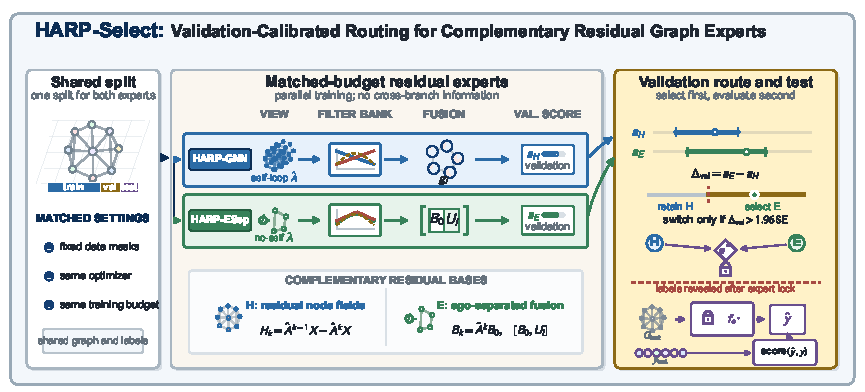
\includegraphics[width=\textwidth]{figures/harp_select_framework.pdf}
}{
  \IfFileExists{figures/harp_select_framework.png}{
    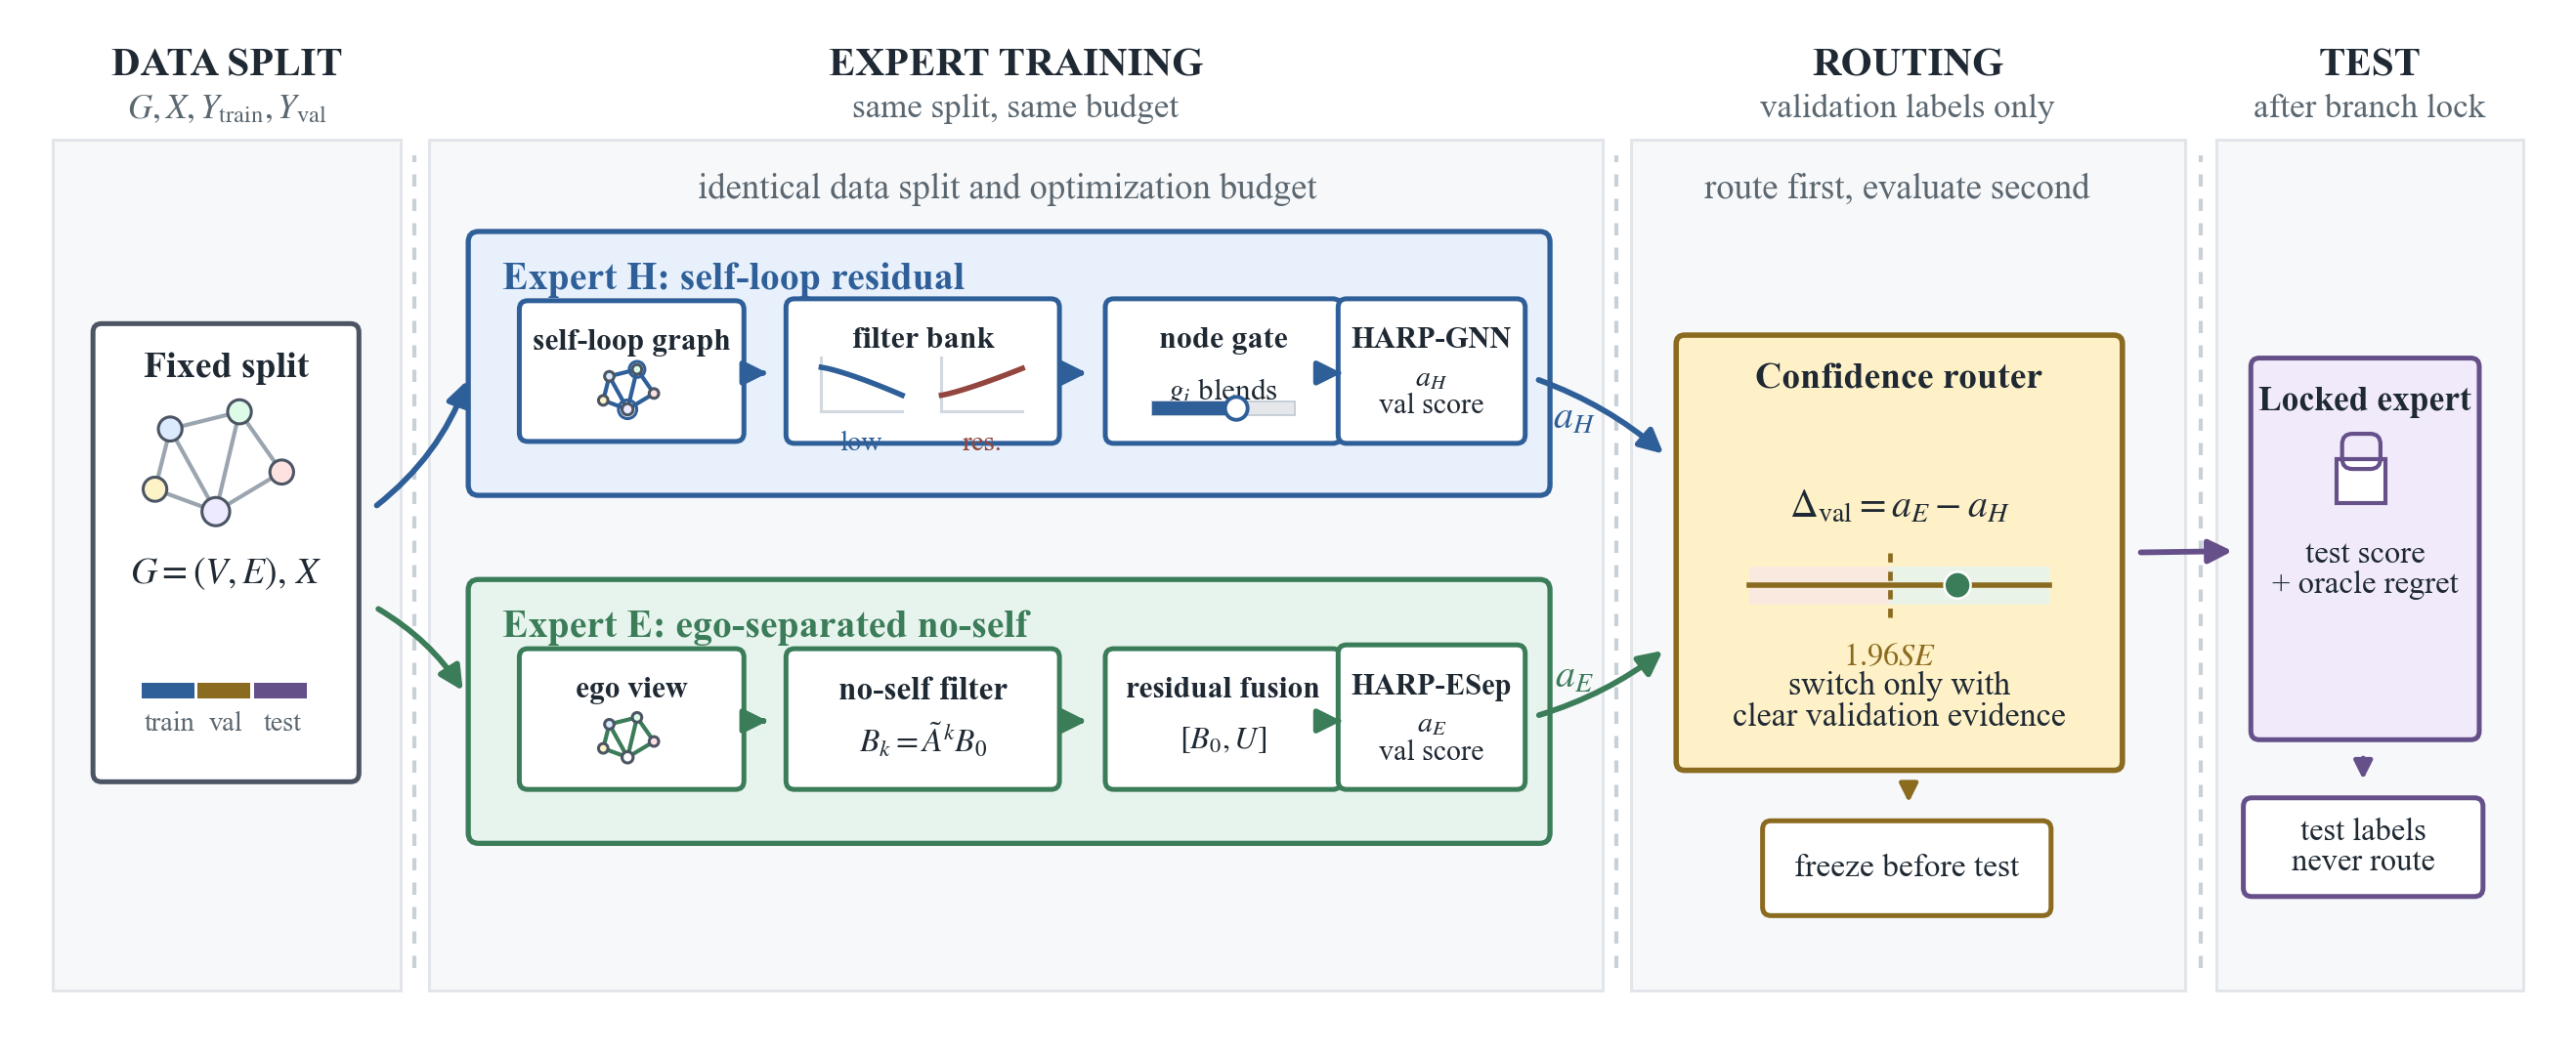
\includegraphics[width=\textwidth]{figures/harp_select_framework.png}
  }{
    \fbox{\rule{0pt}{1.5in}\rule{0.95\textwidth}{0pt}}
  }
}
\caption{\method{} framework. Two residual polynomial experts are trained with the same split and optimization budget. The routing rule uses validation accuracy only and is fixed across datasets; test labels are evaluated only after the branch decision has been made.}
\label{fig:select-framework}
\end{figure*}

\subsection{Self-Loop Residual Expert}

\base{} constructs two signal families.
The low-pass bases are
\begin{equation}
  L_k=\hat{A}^{k}X,\quad k=0,\ldots,K,
\end{equation}
and the high-pass residual bases are
\begin{equation}
  H_k=\hat{A}^{k-1}X-\hat{A}^{k}X,\quad k=1,\ldots,K.
\end{equation}
The branches are mixed with learned polynomial weights:
\begin{equation}
  Z_L=\sum_{k=0}^{K}\alpha_k W_LL_k,\quad
  \alpha=\operatorname{softmax}(\theta_L),
\end{equation}
\begin{equation}
  Z_H=\sum_{k=1}^{K}\beta_k W_HH_k,\quad
  \beta=\operatorname{softmax}(\theta_H).
\end{equation}
The residual branch uses differences between consecutive propagation orders.
Thus $H_1=X-\hat{A}X$ directly captures the local contrast that ordinary averaging removes.
In the eigenbasis of $\hat{A}$, the low-pass response is a nonnegative polynomial
$p_L(\lambda)=\sum_k \alpha_k\lambda^k$, while the residual branch has response
$p_H(\lambda)=(1-\lambda)\sum_{k=1}^{K}\beta_k\lambda^{k-1}$.
The high-pass response therefore vanishes on the constant component $\lambda=1$ and concentrates capacity on deviations that smoothing suppresses.
This gives a simple diagnostic axis: the model is not only adding parameters, but explicitly comparing a smoothing polynomial with its finite-difference complement.

To fuse the branches locally, \base{} computes a label-free feature-variation statistic
\begin{equation}
  r_i=\sigma\left(
  \frac{\|x_i-\operatorname{mean}_{j\in\mathcal{N}(i)}x_j\|_2-\mu}{s+\epsilon}
  \right),
\end{equation}
where $\mu$ and $s$ are graph-level mean and standard deviation.
A gate $g_i=\operatorname{MLP}_g([x_i,r_i])$ produces feature-wise values in $(0,1)$, and the hidden representation is
\begin{equation}
  Z_i=(1-g_i)\odot Z_{L,i}+g_i\odot Z_{H,i},
\end{equation}
followed by normalization, nonlinearity, dropout, and a linear classifier.

\subsection{Ego-Separated Residual Expert}

\esep{} uses the same low/high-pass residual idea but changes the structural prior.
It first encodes ego features,
\begin{equation}
  B_0=\operatorname{ReLU}(XW_E),
\end{equation}
then propagates hidden states with the no-self operator:
\begin{equation}
  B_k=\tilde{A}^{k}B_0,\quad k=1,\ldots,K.
\end{equation}
Low-pass and high-pass hidden views are
\begin{equation}
  U_L=\sum_{k=0}^{K}\gamma_kB_k,\quad
  U_H=\sum_{k=1}^{K}\delta_k(B_{k-1}-B_k),
\end{equation}
with softmax-normalized weights $\gamma$ and $\delta$.
The gate receives ego, low-pass, high-pass, their absolute difference, and the same optional feature-variation signal:
\begin{equation}
  q_i=\operatorname{MLP}_q([B_{0,i},U_{L,i},U_{H,i},|U_{L,i}-U_{H,i}|,r_i]).
\end{equation}
The residual-filtered view is
\begin{equation}
  U_i=(1-q_i)\odot U_{L,i}+q_i\odot U_{H,i}.
\end{equation}
\esep{} classifies from $[B_{0,i},U_i]$.
This preserves ego evidence explicitly while allowing no-self neighborhood signals to contribute through residual filtering.

\section{\method{}: Validation-Calibrated Routing}

The two experts specialize in different regimes, so \method{} treats branch choice as a validation-calibrated model-selection problem.
For each fixed split, both experts are trained independently using the same training labels and optimization budget.
Let $a_H$ and $a_E$ be the validation accuracies of \base{} and \esep, and let $n_{\mathrm{val}}$ be the validation-set size.
The selector computes
\begin{equation}
  \mathrm{SE}=
  \sqrt{\frac{a_H(1-a_H)}{n_{\mathrm{val}}}+
        \frac{a_E(1-a_E)}{n_{\mathrm{val}}}},
\label{eq:selector-se}
\end{equation}
and chooses \esep{} only when
\begin{equation}
  a_E-a_H>1.96\,\mathrm{SE}.
\label{eq:selector-rule}
\end{equation}
Otherwise it retains \base.
Each reported \method{} row logs both branch scores, the validation margin, the threshold, the decision, and oracle regret before any test-label comparison.

The multiplier $1.96$ is the conventional two-sided 95\% normal critical value and is fixed for all datasets.
Because the two validation accuracies are measured on the same validation nodes, the independence approximation can be conservative when errors are positively correlated.
This conservatism is intentional: the selector should move to the no-self expert only when validation evidence is clearly larger than sampling noise.
The tradeoff is that small but stable improvements may be missed, as observed on Amazon-Ratings.

\paragraph{Why not a learned branch gate?}
A single end-to-end gate could in principle interpolate between \base{} and \esep{} at each node.
We tested node-adaptive and logit-blending variants during method development, but they were less reliable: the adaptive branch over-selected the no-self expert on small WebKB graphs and under-selected it on Chameleon and Squirrel, while logit blending was too conservative on the same larger heterophily rows.
The validation selector is therefore intentionally coarse.
It asks for split-level evidence that one structural prior is better for the dataset and training protocol at hand.
This loses node-level flexibility, but it avoids a second learned mechanism whose errors are hard to separate from the graph filter itself.
In a review setting, the coarse selector also gives a cleaner falsification target: if validation margins do not justify a branch switch, the method must retain the self-loop expert and accept the resulting oracle regret.

\section{Experiments}

\paragraph{Questions.}
We ask:
(Q1) Do residual high-pass bases help on heterophilous graphs?
(Q2) Does ego separation repair the larger-heterophily failure mode of the self-loop expert?
(Q3) Can a frozen validation-calibrated selector route between the two without using test labels?
(Q4) Does the evidence survive paired and robust split-level tests?

\paragraph{Datasets.}
We evaluate WebKB Texas, Wisconsin, and Cornell; larger Geom-GCN Actor, Chameleon, and Squirrel; and two external critical-heterophily graphs, Roman-Empire and Amazon-Ratings.
The first six datasets use the standard 10 fixed Geom-GCN splits \cite{pei2020geomgcn}.
Roman-Empire and Amazon-Ratings use the fixed masks supplied by the critical-heterophily benchmark suite \cite{platonov2023critical}.
Table~\ref{tab:critical-data} reports the external graph sizes and split statistics used in the external evaluation.
For the binary critical-heterophily suite, we implement ROC-AUC support and report complete 10-split Minesweeper and Tolokers branch comparisons; Questions remains a loader and metric sanity check and is excluded from the main empirical claims.

\begin{table}[t]
\centering
\caption{External critical-heterophily dataset statistics for split 0. Split lists train/validation/test counts; edges are undirected after symmetrization; Hom. is edge homophily.}
\label{tab:critical-data}
\begingroup
\setlength{\tabcolsep}{2.1pt}
\renewcommand{\arraystretch}{1.08}
\papertablesize
\IfFileExists{tables/critical_heterophily_dataset_stats.tex}{
  \begin{tabular}{lrrrrrrrr}
\toprule
Dataset & Nodes & Edges & Feat. & Classes & Train & Val. & Test & Hom. \\
\midrule
roman-empire & 22,662 & 32,927 & 300 & 18 & 11,331 & 5,665 & 5,666 & 0.047 \\
amazon-ratings & 24,492 & 93,050 & 300 & 5 & 12,246 & 6,123 & 6,123 & 0.380 \\
\bottomrule
\end{tabular}

}{
  \begin{tabular}{lrrrrr}
  \toprule
  Dataset & $|V|$ & $|E|$ & $d/C$ & Split & Hom. \\
  \midrule
  Roman-Emp. & -- & -- & -- & -- & -- \\
  Amazon-Rat. & -- & -- & -- & -- & -- \\
  \bottomrule
  \end{tabular}
}
\endgroup
\end{table}

\paragraph{Baselines.}
The implemented non-HARP baselines are MLP, GCN, SGC, APPNP, MixHop, GPR-GNN, an H2GCN-style separator, and LINKX.
For paired comparisons, each dataset is compared against the strongest implemented non-HARP baseline on that dataset.
This is not a complete heterophily leaderboard: official-code FAGCN, BernNet, and newer methods are outside the implemented comparison, so broad state-of-the-art claims are intentionally out of scope.

\paragraph{Protocol.}
All results are averaged over the 10 fixed splits.
Hyperparameters are selected by validation accuracy.
For \method, branch selection is performed independently on each split using validation labels only.
We report paired $t$-tests, bootstrap 95\% confidence intervals, exact paired sign-flip tests, win/tie/loss counts, and Holm-adjusted $p$-values where available.
Every experiment writes one CSV row per dataset, model, and split, and coverage scripts verify that the expected grid is complete.

\paragraph{Reproducibility controls.}
The artifact treats the reported tables as generated objects rather than manually edited numbers.
Each table in the manuscript is rebuilt from CSV files, and verification scripts check representative means, standard deviations, paired tests, table text, citation keys, anonymous submission markers, and package synchronization.
For the selector, the diagnostic CSV stores both branch validation accuracies, the computed threshold in Eq.~\ref{eq:selector-rule}, the selected branch, and the test accuracy evaluated only after the decision is fixed.
This is deliberately more bookkeeping than a standard benchmark script, but it reduces two common failure modes in heterophily papers: silently changing split coverage and accidentally converting an oracle branch comparison into a claimed method.

\begin{table*}[t]
\centering
\caption{\method{} summary over fixed splits. HARP-Select chooses \esep{} only when its validation advantage exceeds the frozen $1.96\,\mathrm{SE}$ threshold. Oracle is reported only as diagnostic regret, not as a method.}
\label{tab:harp-select}
\begingroup
\setlength{\tabcolsep}{3pt}
\renewcommand{\arraystretch}{1.08}
\papertablesize
\IfFileExists{tables/harp_select_results.tex}{
  \begin{tabular}{lccccc}
\toprule
Dataset & HARP-GNN & HARP-ESep & HARP-Select & Oracle & ESep splits \\
\midrule
actor & 35.08 $\pm$ 1.36 & 35.62 $\pm$ 1.09 & 35.08 $\pm$ 1.36 & 35.86 $\pm$ 0.92 & 0/10 \\
amazon-ratings & 45.43 $\pm$ 0.71 & 45.94 $\pm$ 0.48 & 45.43 $\pm$ 0.71 & 46.18 $\pm$ 0.31 & 0/10 \\
chameleon & 55.90 $\pm$ 2.49 & 63.42 $\pm$ 2.24 & 63.42 $\pm$ 2.24 & 63.42 $\pm$ 2.24 & 10/10 \\
cornell & 74.86 $\pm$ 4.60 & 68.92 $\pm$ 5.87 & 74.86 $\pm$ 4.60 & 75.68 $\pm$ 4.41 & 0/10 \\
roman-empire & 75.76 $\pm$ 0.63 & 78.51 $\pm$ 0.57 & 78.51 $\pm$ 0.57 & 78.51 $\pm$ 0.57 & 10/10 \\
squirrel & 36.66 $\pm$ 1.66 & 46.48 $\pm$ 1.10 & 46.48 $\pm$ 1.10 & 46.48 $\pm$ 1.10 & 10/10 \\
texas & 86.49 $\pm$ 4.59 & 75.41 $\pm$ 4.84 & 86.49 $\pm$ 4.59 & 86.49 $\pm$ 4.59 & 0/10 \\
wisconsin & 87.45 $\pm$ 3.23 & 82.16 $\pm$ 4.57 & 87.45 $\pm$ 3.23 & 87.45 $\pm$ 3.23 & 0/10 \\
\bottomrule
\end{tabular}

}{
  \begin{tabular}{lccccc}
  \toprule
  Dataset & HARP-GNN & HARP-ESep & HARP-Select & Oracle & ESep splits \\
  \midrule
  actor & -- & -- & -- & -- & -- \\
  chameleon & -- & -- & -- & -- & -- \\
  squirrel & -- & -- & -- & -- & -- \\
  texas & -- & -- & -- & -- & -- \\
  wisconsin & -- & -- & -- & -- & -- \\
  cornell & -- & -- & -- & -- & -- \\
  roman-empire & -- & -- & -- & -- & -- \\
  amazon-ratings & -- & -- & -- & -- & -- \\
  \bottomrule
  \end{tabular}
}
\endgroup
\end{table*}

\begin{table*}[t]
\centering
\caption{\method{} versus the strongest implemented non-HARP baseline on the original six fixed-split heterophily datasets. Diff is measured in percentage points over matched splits.}
\label{tab:select-paired}
\begingroup
\setlength{\tabcolsep}{3pt}
\renewcommand{\arraystretch}{1.08}
\papertablesize
\IfFileExists{tables/harp_select_paired_tests.tex}{
  \begin{tabular}{llcccc}
\toprule
Dataset & Best baseline & Baseline & HARP-Select & Diff (pp) & $p$ \\
\midrule
actor & LINKX & 35.67 & 35.08 & -0.59 & 0.245 \\
chameleon & H2GCN & 64.21 & 63.42 & -0.79 & 0.395 \\
cornell & MLP & 76.49 & 74.86 & -1.62 & 0.405 \\
squirrel & LINKX & 45.48 & 46.48 & +1.01 & 0.273 \\
texas & MixHop & 84.59 & 86.49 & +1.89 & 0.132 \\
wisconsin & H2GCN & 85.49 & 87.45 & +1.96 & 0.085 \\
\bottomrule
\end{tabular}

}{
  \begin{tabular}{llcccc}
  \toprule
  Dataset & Best baseline & Baseline & HARP-Select & Diff (pp) & $p$ \\
  \midrule
  actor & -- & -- & -- & -- & -- \\
  chameleon & -- & -- & -- & -- & -- \\
  cornell & -- & -- & -- & -- & -- \\
  squirrel & -- & -- & -- & -- & -- \\
  texas & -- & -- & -- & -- & -- \\
  wisconsin & -- & -- & -- & -- & -- \\
  \bottomrule
  \end{tabular}
}
\endgroup
\end{table*}

\begin{table*}[t]
\centering
\caption{Robust split-level checks for \method{} against the strongest implemented non-HARP baseline. W/T/L counts split-level wins, ties, and losses; Holm $p$ adjusts exact sign-flip tests across the six rows.}
\label{tab:select-robust}
\begingroup
\setlength{\tabcolsep}{2pt}
\renewcommand{\arraystretch}{1.08}
\papertablesize
\IfFileExists{tables/harp_select_robust_tests.tex}{
  \begin{tabular}{llccccc}
\toprule
Dataset & Baseline & Diff (pp) & Bootstrap 95\% CI & W/T/L & Sign-flip $p$ & Holm $p$ \\
\midrule
actor & LINKX & -0.59 & [-1.49, +0.24] & 3/1/6 & 0.242 & 1.000 \\
chameleon & H2GCN & -0.79 & [-2.43, +0.86] & 4/0/6 & 0.383 & 1.000 \\
cornell & MLP & -1.62 & [-5.14, +1.62] & 3/3/4 & 0.359 & 1.000 \\
squirrel & LINKX & +1.01 & [-0.53, +2.72] & 6/0/4 & 0.299 & 1.000 \\
texas & MixHop & +1.89 & [-0.27, +4.05] & 5/3/2 & 0.203 & 1.000 \\
wisconsin & H2GCN & +1.96 & [+0.00, +3.73] & 7/1/2 & 0.125 & 0.750 \\
\bottomrule
\end{tabular}

}{
  \begin{tabular}{llccccc}
  \toprule
  Dataset & Baseline & Diff (pp) & Bootstrap 95\% CI & W/T/L & Sign-flip $p$ & Holm $p$ \\
  \midrule
  actor & -- & -- & -- & -- & -- & -- \\
  chameleon & -- & -- & -- & -- & -- & -- \\
  cornell & -- & -- & -- & -- & -- & -- \\
  squirrel & -- & -- & -- & -- & -- & -- \\
  texas & -- & -- & -- & -- & -- & -- \\
  wisconsin & -- & -- & -- & -- & -- & -- \\
  \bottomrule
  \end{tabular}
}
\endgroup
\end{table*}

\begin{table*}[t]
\centering
\caption{External critical-heterophily comparison against the strongest implemented non-HARP baseline. Best is the strongest non-HARP mean accuracy on that dataset. Diff is \method{} minus that best baseline over paired fixed splits; Holm $p$ is the exact sign-flip value after correction across the two \method{} rows.}
\label{tab:critical-external-main}
\begingroup
\setlength{\tabcolsep}{2.2pt}
\renewcommand{\arraystretch}{1.08}
\papertablesize
\IfFileExists{tables/critical_heterophily_external_main.tex}{
  \begin{tabular}{llcccccc}
\toprule
Dataset & Best non-HARP & Best & HARP-GNN & HARP-ESep & HARP-Select & Diff (pp) & Holm $p$ \\
\midrule
amazon-ratings & LINKX & 46.34 $\pm$ 0.81 & 45.43 $\pm$ 0.71 & 45.94 $\pm$ 0.48 & 45.43 $\pm$ 0.71 & -0.91 & 0.020 \\
roman-empire & H2GCN & 77.73 $\pm$ 0.68 & 75.76 $\pm$ 0.63 & 78.51 $\pm$ 0.57 & 78.51 $\pm$ 0.57 & +0.79 & 0.008 \\
\bottomrule
\end{tabular}

}{
  \begin{tabular}{llcccccc}
  \toprule
  Dataset & Best non-HARP & Best & HARP-GNN & HARP-ESep & HARP-Select & Diff (pp) & Holm $p$ \\
  \midrule
  amazon-ratings & -- & -- & -- & -- & -- & -- & -- \\
  roman-empire & -- & -- & -- & -- & -- & -- & -- \\
  \bottomrule
  \end{tabular}
}
\endgroup
\end{table*}

\begin{table}[t]
\centering
\caption{Binary critical-heterophily branch comparisons under ROC-AUC over 10 fixed splits. Diff is measured in ROC-AUC percentage points and equals \esep{} minus \base.}
\label{tab:binary-critical}
\begingroup
\setlength{\tabcolsep}{2.1pt}
\renewcommand{\arraystretch}{1.08}
\papertablesize
\IfFileExists{tables/critical_heterophily_binary_complete_paired_tests.tex}{
  \begin{tabular*}{\linewidth}{@{\extracolsep{\fill}}lccccc@{}}
\toprule
Dataset & HARP-GNN & HARP-ESep & Diff (pp) & $n$ & $p$ \\
\midrule
minesweeper & 88.18 $\pm$ 0.84 & 89.64 $\pm$ 0.67 & +1.45 & 10 & $<0.001$ \\
tolokers & 82.79 $\pm$ 0.83 & 79.22 $\pm$ 0.70 & -3.56 & 10 & $<0.001$ \\
\bottomrule
\end{tabular*}

}{
  \begin{tabular}{lccccc}
  \toprule
  Dataset & HARP-GNN & HARP-ESep & Diff (pp) & $n$ & $p$ \\
  \midrule
  minesweeper & -- & -- & -- & -- & -- \\
  tolokers & -- & -- & -- & -- & -- \\
  \bottomrule
  \end{tabular}
}
\endgroup
\end{table}

\subsection{Main Results}

Table~\ref{tab:harp-select} shows the specialization pattern.
On Texas and Wisconsin, the self-loop expert remains strongest among the two HARP branches, so \method{} retains \base{} on all splits.
On Chameleon and Squirrel, \esep{} is much stronger and the selector routes all splits to it.
On Actor, the ego-separated branch has a small mean advantage, but its validation gains do not exceed the fixed confidence threshold, so \method{} conservatively keeps \base.
This is the intended behavior: the selector moves only when validation evidence is large relative to the validation-set uncertainty.

The original six-dataset comparison in Table~\ref{tab:select-paired} is balanced rather than dominant.
\method{} is positive against the strongest implemented non-HARP baseline on Texas, Wisconsin, and Squirrel, and negative on Cornell, Actor, and Chameleon.
None of the paired $t$-tests are significant at $p<0.05$.
In particular, current positive margins are not significant at $p<0.05$.
The robust checks in Table~\ref{tab:select-robust} lead to the same conclusion: exact sign-flip tests with Holm correction produce no significant row.
This matters because the original self-loop expert had significant negative margins on Chameleon and Squirrel; \method{} removes those significant deficits, but it does not create a significant superiority claim.

External validation becomes sharper after adding non-HARP baselines.
On Roman-Empire, \esep{} improves over \base{} by 2.75 percentage points, and Table~\ref{tab:critical-external-main} shows that \method{} also exceeds the strongest implemented non-HARP baseline, H2GCN, by 0.79 points with 10/10 split wins and Holm-corrected exact sign-flip $p=0.008$.
The frozen selector routes all Roman-Empire splits to \esep.
On Amazon-Ratings, \esep{} has a smaller 0.50 point mean advantage over \base{} that is not significant, while LINKX is the strongest implemented baseline.
\method{} keeps \base{} on all splits and trails LINKX by 0.91 points, exposing a real limitation: the current expert library lacks a LINKX-like adjacency expert for this graph.
The binary critical-heterophily rows in Table~\ref{tab:binary-critical} sharpen the mechanism rather than giving a uniform gain.
On Minesweeper, \esep{} reaches 89.64 ROC-AUC versus 88.18 for \base{}, a +1.45 point paired difference with 10/10 split wins.
On Tolokers, the direction reverses: \base{} reaches 82.79 while \esep{} reaches 79.22, a -3.56 point difference with 0/10 split wins.
Both rows have Holm-corrected exact sign-flip $p=0.004$.
We treat this as branch evidence only; the validation selector uses an accuracy-derived uncertainty rule and is therefore not applied to ROC-AUC datasets.

\subsection{Mechanistic Evidence}

Figure~\ref{fig:harp-block} depicts the internal residual polynomial block used by the self-loop expert.

\begin{figure}[t]
\centering
\IfFileExists{figures/harp_framework.pdf}{
  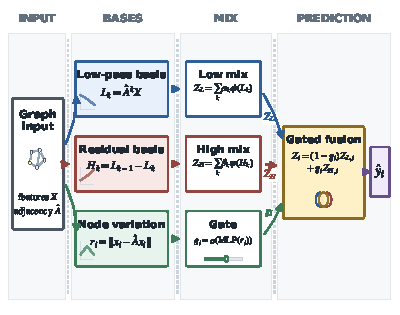
\includegraphics[width=\linewidth]{figures/harp_framework.pdf}
}{
  \IfFileExists{figures/harp_framework.png}{
    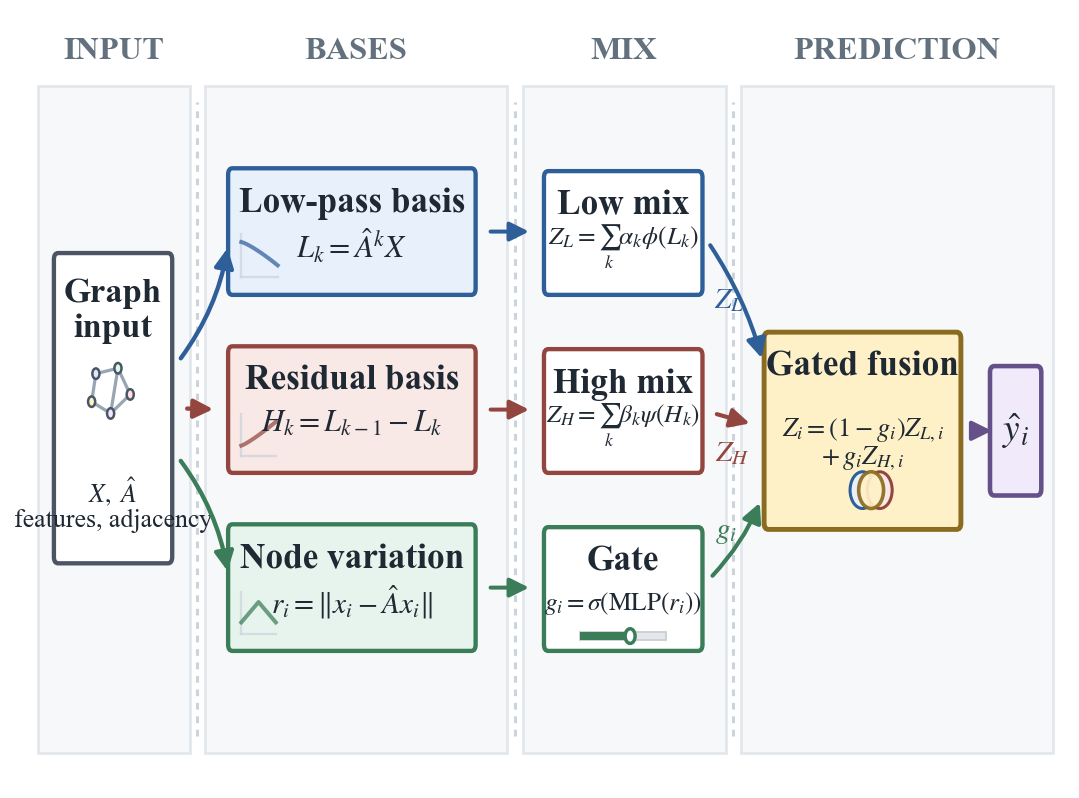
\includegraphics[width=\linewidth]{figures/harp_framework.png}
  }{
    \fbox{\rule{0pt}{1.35in}\rule{0.92\linewidth}{0pt}}
  }
}
\caption{\base{} internal residual polynomial block. \method{} uses this self-loop expert as one branch and pairs it with an ego-separated no-self version of the same residual filtering idea.}
\label{fig:harp-block}
\end{figure}

\begin{table*}[t]
\centering
\caption{WebKB ablations isolating multi-hop mixing, low/high-pass residual branches, and the gate signal.}
\label{tab:ablation}
\begingroup
\setlength{\tabcolsep}{3pt}
\renewcommand{\arraystretch}{1.08}
\papertablesize
\IfFileExists{tables/webkb_ablation_results.tex}{
  \begin{tabular*}{0.94\linewidth}{@{\extracolsep{\fill}}lccccc@{}}
\toprule
Dataset & MixHop & HARP-GNN & HARP-Low & HARP-High & HARP-NoSignal \\
\midrule
cornell & 74.59 $\pm$ 3.17 & 74.86 $\pm$ 4.60 & 51.35 $\pm$ 11.18 & 72.43 $\pm$ 6.34 & \textbf{75.41 $\pm$ 4.12} \\
texas & 84.59 $\pm$ 4.60 & \textbf{86.49 $\pm$ 4.59} & 62.43 $\pm$ 7.69 & 81.35 $\pm$ 6.43 & 85.14 $\pm$ 6.40 \\
wisconsin & 83.73 $\pm$ 5.47 & \textbf{87.45 $\pm$ 3.23} & 75.49 $\pm$ 6.22 & 79.02 $\pm$ 4.90 & \textbf{87.45 $\pm$ 4.26} \\
\bottomrule
\end{tabular*}

}{
  \begin{tabular}{lccccc}
  \toprule
  Dataset & MixHop & HARP-GNN & HARP-Low & HARP-High & HARP-NoSignal \\
  \midrule
  Texas & -- & -- & -- & -- & -- \\
  Wisconsin & -- & -- & -- & -- & -- \\
  Cornell & -- & -- & -- & -- & -- \\
  \bottomrule
  \end{tabular}
}
\endgroup
\end{table*}

\begin{table*}[t]
\centering
\caption{Learned \base{} polynomial weights on WebKB. Low-pass bases are $L_0,\ldots,L_3$ and high-pass residual bases are $H_1,\ldots,H_3$.}
\label{tab:filter-weights}
\begingroup
\setlength{\tabcolsep}{2pt}
\renewcommand{\arraystretch}{1.08}
\papertablesize
\IfFileExists{tables/webkb_filter_weights.tex}{
  \begin{tabular*}{0.94\linewidth}{@{\extracolsep{\fill}}lccccccc@{}}
\toprule
Dataset & L0 & L1 & L2 & L3 & H1 & H2 & H3 \\
\midrule
cornell & 0.317 $\pm$ 0.015 & 0.236 $\pm$ 0.017 & 0.223 $\pm$ 0.010 & 0.223 $\pm$ 0.010 & 0.473 $\pm$ 0.054 & 0.265 $\pm$ 0.025 & 0.263 $\pm$ 0.029 \\
texas & 0.301 $\pm$ 0.017 & 0.263 $\pm$ 0.023 & 0.218 $\pm$ 0.012 & 0.218 $\pm$ 0.010 & 0.481 $\pm$ 0.047 & 0.262 $\pm$ 0.022 & 0.257 $\pm$ 0.025 \\
wisconsin & 0.316 $\pm$ 0.012 & 0.227 $\pm$ 0.009 & 0.230 $\pm$ 0.008 & 0.227 $\pm$ 0.005 & 0.459 $\pm$ 0.022 & 0.277 $\pm$ 0.016 & 0.264 $\pm$ 0.008 \\
\bottomrule
\end{tabular*}

}{
  \begin{tabular}{lccccccc}
  \toprule
  Dataset & L0 & L1 & L2 & L3 & H1 & H2 & H3 \\
  \midrule
  Texas & -- & -- & -- & -- & -- & -- & -- \\
  Wisconsin & -- & -- & -- & -- & -- & -- & -- \\
  Cornell & -- & -- & -- & -- & -- & -- & -- \\
  \bottomrule
  \end{tabular}
}
\endgroup
\end{table*}

The ablations in Table~\ref{tab:ablation} support the residual interpretation.
Low-pass-only HARP is weak on WebKB, while high-pass residual filtering recovers much of the lost performance.
The full feature-wise gate is strongest on Texas and competitive on Wisconsin, although the no-signal variant remains close and is slightly better on Cornell.
Thus the safest mechanistic claim is that residual low/high-pass fusion is useful; the handcrafted feature-variation signal is a bounded hypothesis rather than the sole source of the gain.
Table~\ref{tab:filter-weights} further shows that learned filters allocate substantial mass to first-order high-pass residuals on WebKB, consistent with the idea that local contrastive evidence is important under heterophily.

\subsection{Failure Modes}

The strongest negative evidence is as important as the positive branch result.
On WebKB, globally replacing \base{} with the no-self expert is harmful, which means ego separation is not a universal cure for heterophily.
On Actor, \esep{} has a mild mean advantage over \base{}, but the validation margin is too small to trigger the frozen selector; this produces a conservative decision rather than a hidden oracle.
On Amazon-Ratings, the same conservatism misses a small non-significant \esep{} advantage.
Tolokers points in the opposite direction from Minesweeper: under complete 10-split ROC-AUC evaluation, every paired split favors the self-loop expert.
These failures clarify the intended use of \method{}.
It is most appropriate when two structural priors have visibly different validation behavior; it is not a replacement for stronger single-model architectures when validation evidence is weak or when deployment requires one compact model.

\subsection{Cost}

\method{} trains both experts before validation routing.
The artifact's recorded CPU wall-clock trace gives a macro mean two-expert cost of 95.0 seconds per split across the eight selector datasets, 1.72$\times$ the self-loop expert on average and 2.11 hours across all 80 selector branch runs.
This is acceptable for an auditable benchmark study but not an efficiency claim.
A natural next step is to distill the selected expert into a shared encoder or train a cheaper selector before full expert training.

\section{Limitations and Ethics}

This manuscript does not claim final state-of-the-art performance.
The main limitation is baseline coverage.
The implemented comparison includes MLP, GCN, SGC, APPNP, MixHop, GPR-GNN, an H2GCN-style separator, and LINKX, but not official-code FAGCN, BernNet, or newer 2025--2026 heterophily methods.
The external Roman-Empire result is therefore evidence for the HARP branch design, not a complete leaderboard claim.
The critical-heterophily ROC-AUC evaluation now includes complete Minesweeper and Tolokers branch comparisons, while Questions remains a loader and metric sanity check rather than a reported main claim.

The selector is conservative by design.
This avoids overreacting to validation noise, but misses small advantages such as Amazon-Ratings.
It also doubles training cost and selects at the split level rather than learning a single deployable architecture.
These are scientific limitations, not incidental engineering details, and we report them explicitly.

This work uses public benchmark datasets for node classification.
As with all graph learning systems, deployment on social, educational, or recommendation networks could amplify measurement bias or expose sensitive relational structure.
The artifact is intended for benchmark research, and any applied use should include dataset-specific privacy and fairness review.

\paragraph{Practical implications.}
The experiments suggest a pragmatic workflow for new heterophilous graphs.
First, compare a self-loop residual expert and an ego-separated no-self expert on the prescribed validation split instead of choosing a propagation convention by convention.
Second, inspect the validation margin together with its uncertainty, because small branch differences can reverse across splits and should not be promoted to architectural claims.
Third, report the selector regret against the branch oracle even when the selected model is competitive; regret is the clearest diagnostic of whether the routing threshold is too conservative.
Finally, separate branch evidence from selector evidence.
Minesweeper and Roman-Empire show that the no-self residual expert can be the better branch, while Tolokers and WebKB warn that the same branch can be worse elsewhere.
The scientific value of \method{} is precisely this separation: it makes the structural prior, validation decision, and test consequence visible as distinct quantities.

\paragraph{Interpreting mixed evidence.}
The empirical picture is intentionally uneven.
This matters for a heterophily paper because a method that only reports its best branch can obscure the central modeling question: which neighborhood relation is being trusted?
\method{} makes that question explicit.
The WebKB rows show that self information remains important when local labels are noisy but ego features carry useful class evidence.
The Roman-Empire and Minesweeper rows show the opposite risk: retaining the ego state inside every propagation path can dilute contrastive neighborhood evidence.
Actor, Chameleon, and Squirrel then act as useful stress tests because neither a self-loop residual expert nor a no-self expert should be expected to repair every benchmark regime.
Reading these rows together gives a narrower but more useful claim than a leaderboard statement: branch identity is itself an experimental variable, and freezing the branch decision before test evaluation turns that variable into an auditable part of the method.

\paragraph{Audit trail as a method component.}
The selector is small enough that each decision can be inspected after the run.
For every split we can report the validation margin, its standard-error threshold, the selected branch, the oracle branch, and the resulting regret.
This audit trail is not only a reproducibility convenience.
It also prevents three common failure modes in graph benchmark papers.
First, it separates architecture search from test-set reporting.
Second, it exposes datasets where a branch looks promising on average but is too unstable to select confidently on a fixed split.
Third, it reveals when the proposed family is simply missing a stronger expert, as in the larger Geom-GCN deficits.
\paragraph{Scope for extensions.}
The present implementation keeps two residual polynomial experts and a conservative graph-level selector.
This is a deliberate restriction rather than an assumption that two experts are sufficient.
The same evaluation protocol could support richer expert libraries, node-level confidence rules, or cheaper distilled selectors, but those variants should be judged under the same frozen-split discipline.
In particular, a learned gate should be compared against the transparent selector on regret, calibration, and stability, not only on mean accuracy.
Likewise, adding recent heterophily baselines should preserve the distinction between primary claims, diagnostic branches, and non-claimed sanity checks.
The goal is to make subsequent evaluations scientifically harder to overclaim: stronger baselines may reduce the apparent advantage, but they will also clarify whether branch-aware residual filtering solves a reproducible modeling problem.

\section{Conclusion}

\method{} frames heterophilous graph learning as a choice between residual polynomial experts rather than a commitment to one universal graph filter.
The self-loop expert is useful on WebKB-style graphs, the ego-separated no-self expert repairs larger heterophily failures and improves Roman-Empire under paired tests, and a frozen validation-calibrated selector routes between them without test labels.
The evidence is deliberately bounded: it supports an auditable specialist-and-routing formulation rather than a universal heterophily leaderboard result.
This boundedness is useful because it identifies the next scientific tests: stronger official baselines, the remaining ROC-AUC critical datasets, and cheaper deployable selectors.
The broader methodological lesson is that heterophily mechanisms should be evaluated with the same visibility as their accuracy numbers.
When a model changes the role of self-loops, high-pass residuals, gates, or branch selectors, the paper should show how that choice was made before test evaluation and where the same choice fails.
\method{} follows this discipline by turning branch selection into a recorded decision rule rather than an implicit hyperparameter.
New datasets, experts, and learned gates can be added under the same audit trail by reporting validation margins, thresholds, selected branches, oracle regret, and final paired evidence.
Under that standard, a branch-aware graph model should not only fit labels on a benchmark; it should explain which structural evidence it trusted and why that trust was justified before seeing the test labels.

\clearpage
\typeout{HARP_REFERENCES_START_PAGE=\thepage}
\bibliography{references,references_additions}

\end{document}
